\documentclass[11pt]{article}
\usepackage{acl}
\usepackage{times}
\usepackage{latexsym}
\usepackage[T1]{fontenc}
\usepackage[utf8]{inputenc}
\usepackage{microtype}
\usepackage{inconsolata}
\usepackage{graphicx}
\usepackage{booktabs}
\usepackage{amsmath}
\usepackage{amssymb}
\usepackage{tikz}
\usetikzlibrary{arrows.meta,positioning}

\title{CLAE: A Continuous-Latent Autoencoder for Bengali Speech}
\author{Anonymous authors}

\begin{document}
\maketitle

\begin{abstract}
We study a continuous-latent autoencoder for 16~kHz Bengali speech that jointly supports waveform reconstruction and frozen-feature evaluation. The full model has 23.80M parameters; its 15.29M-parameter frontend and encoder produce a 256-dimensional representation $z$ at 12.5 frames/s. A separate per-frame projector maps $z$ to a 64-dimensional space $p$. Training combines waveform reconstruction evaluated by an 80-bin log-mel loss, non-contrastive global/local view consistency in $p$, and Variance-Invariance-Sketching Regularization (VISReg) in $p$. At the selected 210k-step checkpoint, reconstruction on 400 held-out Common Voice Bengali clips gives MR-STFT 0.747, STOI 0.850, ESTOI 0.762, and PESQ-WB 2.146; frozen $z$ features also support the reported emotion, age, gender, and speaker probes. A separate matched 25k-step study shows that removing reconstruction worsens reconstruction metrics and two temporal-emotion probes in this setting. At the same 25k checkpoint budget, the 12.5~Hz model and Mimi with eight quantizers exhibit a metric-dependent reconstruction trade-off. These results are single-seed point estimates and objective proxy measurements; we make no claim about statistical significance or subjective audio quality.
\end{abstract}

\section{Introduction}

Continuous speech representations offer a different design point from discrete neural codec tokens. They avoid a quantization bottleneck, but they do not by themselves provide a bitrate or a token sequence suitable for entropy coding. This paper investigates a narrower question: whether a compact, low-frame-rate continuous representation can jointly support waveform reconstruction and selected frozen-feature probes for Bengali speech.

We present CLAE, a 23.80M-parameter continuous-latent autoencoder trained on an approximately 2,000-hour inventory assembled from four Bengali speech sources. The encoder produces a 256-dimensional frame-level representation $z$ at 12.5~Hz. The decoder and all downstream probes consume $z$. A distinct 64-dimensional projector output $p$ is used only by two representation objectives: direct global/local view consistency and Variance-Invariance-Sketching Regularization (VISReg; \citealp{wu2026visreg}). Reconstruction remains a central training branch: the decoder generates a waveform from a corrupted copy of $z$, and the generated waveform is compared with the clean source in an 80-bin log-mel domain.

The contribution is empirical and implementation-specific. We provide: (i) a continuous 12.5~Hz Bengali speech autoencoder; (ii) a combination of waveform reconstruction, non-contrastive view consistency, and frame-level VISReg; (iii) a Conformer-derived encoder with a project adaptation of Manifold-Constrained Hyper-Connections (mHC); and (iv) completed evaluations of the selected 210k-step checkpoint together with a matched 25k-step ablation suite. We do not claim that the individual components are new, that the representation is a deployment codec, or that the reported tasks establish broad language or population coverage.

\section{Related Work}

\paragraph{Joint-embedding learning.}
Image JEPA introduced prediction in representation space using distinct context and target pathways \citep{assran2023ijepa}; A-JEPA adapted masked-target JEPA ideas to audio \citep{fei2023ajepa}. LeJEPA instead studies direct view agreement with isotropic-Gaussian regularization \citep{balestriero2025lejepa}. CLAE is closest to the latter at a conceptual level, but differs in domain, waveform view construction, grouped consistency loss, frame-level population, regularizer, and the addition of reconstruction. In particular, CLAE has one shared encoder and no target encoder, exponential moving average, learned predictor, stop-gradient target path, or negative pairs.

\paragraph{Distribution regularization.}
VICReg combines invariance, per-dimension variance control, and covariance regularization \citep{bardes2022vicreg}. VISReg retains explicit center and scale terms but replaces covariance control with random one-dimensional projections whose sorted samples are matched to Gaussian quantiles \citep{wu2026visreg}. We use the exact name Variance-Invariance-Sketching Regularization. The project adopted the recent VISReg preprint in July 2026 and applies a local, frame-level adaptation described in Section~\ref{sec:visreg}; no controlled VISReg-versus-SIGReg experiment is available.

\paragraph{Continuous and discrete audio representations.}
Continuous Audio Language Models use a continuous variational bottleneck, KL regularization, additional speech distillation, and generative next-frame modeling \citep{rouard2025calm}; those components are not used here. UniWav studies joint representation and generation objectives for speech \citep{liu2025uniwav}. By contrast, UniAudio and UniTok-Audio illustrate autoregressive generation over discrete audio tokens \citep{yang2024uniaudio,liu2025unitokaudio}. Neural codecs such as SoundStream and EnCodec learn quantized, bitrate-controlled representations \citep{zeghidour2021soundstream,defossez2023encodec}. Mimi, introduced with Moshi, is the controlled reconstruction baseline used in our 25k study \citep{defossez2024moshi}. CLAE's continuous floating-point latent is neither quantized nor entropy-coded, so its scalar rate is not directly comparable to codec bitrate.

\paragraph{Sequence encoder and residual connections.}
The encoder builds on the Conformer macaron block \citep{gulati2020conformer}. Its local class name refers to FastConformer, but it does not implement the published architecture's complete downsampling and scalable/local-attention design \citep{rekesh2023fastconformer}; we therefore call it a Conformer-derived encoder. Selected layers use a project adaptation of Manifold-Constrained Hyper-Connections \citep{xie2025mhc}, not a codebook, clustering method, or quantizer.

\section{Method}

\subsection{Architecture}

For a 16~kHz mono waveform $x$, the convolutional frontend has five Conv1D stages with channels $[128,256,384,512,512]$, kernels $[10,8,8,4,4]$, and strides $[5,4,4,4,4]$, with GroupNorm and GELU. Its total stride is 1,280 samples, yielding approximately 12.5 frames/s. An eight-layer, 256-dimensional Conformer-derived encoder uses eight attention heads, a 1,024-dimensional feed-forward sublayer, rotary full self-attention, macaron feed-forward modules, a 9-tap convolution branch, dropout 0.1, and squeeze-and-excitation. It produces
\begin{equation}
z = E(F(x)), \qquad z\in\mathbb{R}^{T'\times256}.
\end{equation}
A per-frame MLP projector with dimensions $256\rightarrow512\rightarrow64$ produces $p=P(z)$. The decoder and downstream frozen-feature probes use $z$, whereas the consistency and VISReg objectives use $p$.

The FiLM-conditioned waveform decoder starts with 768 channels, reverses the frontend with strides $[4,4,4,4,5]$, and uses two residual blocks per upsampling stage with dilations $[1,3,9]$. The full training model has 23,803,125 parameters. The frontend, encoder, projector, and decoder contain 2,890,240, 12,403,220, 165,440, and 8,344,225 parameters, respectively. The frozen frontend--encoder feature extractor therefore contains 15,293,460 parameters.

\begin{figure*}[t]
\centering
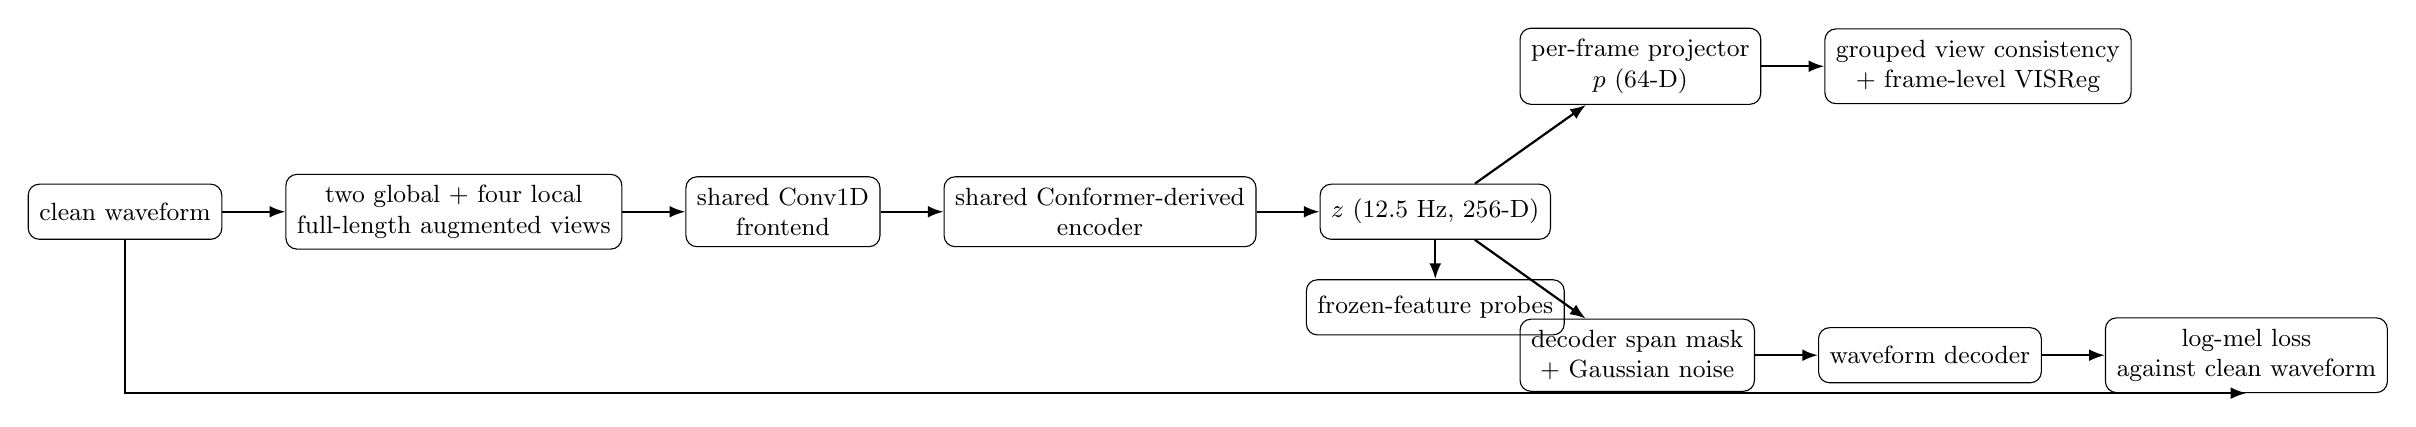
\begin{tikzpicture}[
  node distance=5mm and 8mm,
  box/.style={draw,rounded corners,align=center,minimum height=7mm,inner sep=4pt,font=\small},
  arr/.style={-{Latex[length=2mm]},thick}
]
\node[box] (wave) {clean waveform};
\node[box,right=of wave] (views) {two global + four local\\full-length augmented views};
\node[box,right=of views] (front) {shared Conv1D\\frontend};
\node[box,right=of front] (enc) {shared Conformer-derived\\encoder};
\node[box,right=of enc] (z) {$z$ (12.5 Hz, 256-D)};
\node[box,below right=10mm and -4mm of z] (decnoise) {decoder span mask\\+ Gaussian noise};
\node[box,right=of decnoise] (dec) {waveform decoder};
\node[box,right=of dec] (mel) {log-mel loss\\against clean waveform};
\node[box,above right=10mm and -4mm of z] (proj) {per-frame projector\\$p$ (64-D)};
\node[box,right=of proj] (repr) {grouped view consistency\\+ frame-level VISReg};
\node[box,below=of z] (probes) {frozen-feature probes};
\draw[arr] (wave)--(views);
\draw[arr] (views)--(front);
\draw[arr] (front)--(enc);
\draw[arr] (enc)--(z);
\draw[arr] (z)--(proj);
\draw[arr] (proj)--(repr);
\draw[arr] (z)--(decnoise);
\draw[arr] (decnoise)--(dec);
\draw[arr] (dec)--(mel);
\draw[arr] (wave.south) |- (mel.south);
\draw[arr] (z)--(probes);
\end{tikzpicture}
\caption{Implemented training and evaluation path. All six views share the same frontend, encoder, and projector. Local views are full-length three-second views with stronger augmentation and masking, not shorter temporal crops. Decoder corruption is applied after the encoder and is separate from view construction.}
\label{fig:architecture}
\end{figure*}

\subsection{Waveform views and consistency objective}

Training normally samples three-second source segments. Two global views receive independently sampled waveform augmentation. Four local views remain full-length three-second waveforms but receive stronger waveform augmentation and waveform-aligned span masking; their frontend features can receive an additional independent frame mask. All six views pass through the same frontend, encoder, and projector.

Let $p_g$ and $p_l$ denote projector features grouped into global and local views. For each example and frame, the center $\bar p_g$ is the mean of the two global projector features. The implemented consistency loss is
\begin{equation}
\mathcal{L}_{\mathrm{view}}=
\operatorname{mean}\!\left[(p_g-\bar p_g)^2\right]
+\operatorname{mean}\!\left[(p_l-\bar p_g)^2\right].
\label{eq:view}
\end{equation}
The two group means are added, so global and local groups have equal aggregate contribution despite containing two and four views. This is non-contrastive global/local view consistency, not context-to-target or masked-region prediction.

\subsection{VISReg adaptation}
\label{sec:visreg}

The local VISReg implementation flattens projector frames from all views and examples into one population; it does not pool them. Under distributed training, the population is gathered across workers. Its effective shape is $N=1$, $B=T'VB_{\mathrm{global}}$, and $D=64$. For population points $q_i\in\mathbb{R}^D$, it penalizes the population mean, centers the points, computes a per-dimension RMS scale with division by $\sqrt{B}$, and penalizes deviation from unit scale. Normalization uses a detached scale. On every forward pass, 256 normalized Gaussian directions are sampled. Values projected onto each direction are sorted and matched to standard-normal quantiles $\Phi^{-1}(i/(B+1))$. Center, scale, and projected-distribution shape terms have equal internal weight.

This implements the core VISReg center/scale/shape construction with project-specific frame-level and distributed adaptations. The version used by the 210k checkpoint is the repository implementation at commit \texttt{35be6652f7a2fc569ff318838e36143f2de5232d}. Relative to the later upstream implementation, it gathers across workers, adds $10^{-6}$ to scale rather than using a lower clamp, fixes equal internal weights, and casts cached target quantiles to the activation dtype. The main run uses BF16. We do not describe this version as identical to the current upstream implementation.

\subsection{Reconstruction and total objective}

The decoder receives $z$ from the first global view. Before decoding, an independent span mask removes 50\% of frames in spans of 4--24 frames and Gaussian noise with standard deviation 0.03 is added. The target remains the clean source waveform. The decoder outputs a waveform, which is compared with the clean waveform using an 80-bin log-mel loss with FFT size 1,024, window length 1,024, hop length 256, a Hann window, magnitude weight 1.0, log-magnitude weight 1.0, and spectral-convergence weight 0. Multi-resolution STFT code exists but is not an additional training objective for the selected run.

The selected objective is
\begin{equation}
\mathcal{L}_{\mathrm{total}}=
1.0\mathcal{L}_{\mathrm{mel}}+
0.3\mathcal{L}_{\mathrm{view}}+
0.7\mathcal{L}_{\mathrm{VISReg}}.
\end{equation}
These values are coefficients for losses with different scales; 0.7 is not a percentage of the total objective. Vector quantization, a variational bottleneck, KL divergence, adversarial loss, feature matching, and autoregressive prediction are inactive in the selected run.

\subsection{mHC adaptation}

At zero-indexed encoder layers 2 and 5, mHC widens the residual path to two streams. It applies learned static pre/post mixing and a Sinkhorn-constrained residual matrix with identity blending, uses ten Sinkhorn iterations, wraps complete encoder layers, and returns to one stream by a project-specific uniform mean readout. These choices adapt the reference mHC design rather than reproduce its complete large-model implementation. Section~\ref{sec:ablation} reports mixed, probe-dependent evidence for this component.

\section{Data and Training}

The documented inventory contains 1,052,178 Common Voice Bengali utterances, 218,703 OpenSLR-53 utterances, 21,313 regspeech12 utterances, and 17,882 shrutilipi utterances, for 1,310,076 records in total. The fixed split contains 1,244,572 training and 65,504 validation records. Unique duration is approximately 2,000 hours; no exact audited duration is available. Common Voice and OpenSLR-53 both contribute to pretraining, so evaluations on those sources are in-domain or transductive frozen-feature evaluations. The inventory does not establish demographic or dialect balance, and no deduplication or train--evaluation leakage audit was performed. SUBESCO \citep{sultana2021subesco}, used for emotion evaluation, is absent from the documented training inventory.

The selected checkpoint comes from run \texttt{large-2kh-packed-210k-tail-lr-1e4}.\footnote{Repository-relative checkpoint path: \nolinkurl{runs/large-2kh-packed-210k-tail-lr-1e4/checkpoints/last.pt}.} Training uses BF16, AdamW, batch size 42, gradient accumulation over four batches, and gradient clipping at 1.0. Training was resumed in segments with manual base-learning-rate reductions: the packed continuation used the repository base configuration, a later continuation used $5\times10^{-4}$, and the tail used $10^{-4}$ with a 300k scheduler horizon before the final maximum was set to 210k. The scheduler is reconstructed from the completed step and the active resume configuration rather than restored as independent state; this is not one uninterrupted default cosine schedule.

The effective batch is 168 source segments per optimizer step. At 210,000 steps this corresponds to 35.28M sampled source segments, or 105.84M seconds (29,400 hours) of nominal source-audio exposure. It is also about 28.35 training-manifest-equivalent sampled utterance counts. These are exposure-equivalent quantities, not unique examples or duration: augmentation, random cropping, packed-data shuffling, and repeated sampling alter what is observed. The six representation views increase computation but are not six independently sampled source recordings.

There is no active in-loop validation. Configuration fields for a validation manifest, evaluation interval, and validation batches do not trigger validation in the training path. W\&B records training provenance and diagnostics; its curves are not validation curves and are not used here as evidence of generalization.

\section{Evaluation}

We report only completed artifacts that identify the checkpoint, data, protocol, and metric. The selected 210k checkpoint is evaluated separately from the matched 25k ablations; their absolute scores should not be interpreted as a checkpoint-matched comparison. Reconstruction metrics are objective proxies. PESQ \citep{rix2001pesq}, STOI \citep{taal2010stoi}, ESTOI \citep{jensen2016estoi}, and MR-STFT \citep{yamamoto2020parallelwavegan} do not substitute for listener judgments.

\subsection{Selected 210k checkpoint}

Table~\ref{tab:main210k} reports the complete existing artifacts selected for the main analysis. Reconstruction uses a fixed order of 400 three-second Common Voice Bengali validation clips and FP32 inference. Classification probes keep the frontend and encoder frozen. Emotion, age, and gender use speaker-disjoint folds. Closed-set speaker identification holds out utterances from the same enrolled speakers. Speaker verification uses cosine-scored all-pairs trials, which is a diagnostic rather than a standard enrollment/test benchmark. To keep the reporting consistent with the compact evaluation setting, Table~\ref{tab:main210k} gives the fixed seed-0 point estimate for learned probes; reconstruction and verification have no probe seed.

\begin{table*}[t]
\centering
\footnotesize
\setlength{\tabcolsep}{3.4pt}
\begin{tabular}{@{}lllr@{}}
\toprule
Task & Data and protocol & Metric & Result \\
\midrule
Reconstruction & Common Voice Bengali, fixed 400 clips & MR-STFT $\downarrow$ & 0.747 \\
 & & STOI $\uparrow$ / ESTOI $\uparrow$ & 0.850 / 0.762 \\
 & & PESQ-WB $\uparrow$ & 2.146 \\
Emotion (linear) & SUBESCO, 5 speaker-group folds, 7,000 utt. & macro-F1 $\uparrow$ & 0.482 \\
Emotion (temp. attention) & SUBESCO, 1,708 train / 392 held-out utt. & macro-F1 $\uparrow$ & 0.359 \\
Emotion (temp. Transformer) & SUBESCO, 4 speaker-group folds, 7,000 utt. & macro-F1 $\uparrow$ & 0.516 \\
Age & Common Voice, 5 speaker-group folds, 15,475 utt. & balanced acc. / macro-F1 $\uparrow$ & 0.259 / 0.216 \\
Gender & Common Voice, 5 speaker-group folds, 15,690 utt. & balanced acc. / macro-F1 $\uparrow$ & 0.954 / 0.928 \\
Closed-set speaker ID & 167 speakers, 666 train / 334 test utt. & accuracy $\uparrow$ & 0.656 \\
Speaker verification & 334 speakers, 2,000 utt., all-pairs, mean+std & EER / minDCF $\downarrow$ & 0.276 / 0.988 \\
\bottomrule
\end{tabular}
\caption{Completed evaluations for the selected 210k checkpoint. ``Temp.'' denotes temporal attention or the temporal Transformer, respectively. Probe values are fixed seed-0 point estimates. The tasks use different datasets and protocols and should not be combined into an overall ranking.}
\label{tab:main210k}
\end{table*}

The table establishes performance only under the stated protocols. Common Voice results are transductive because that source also appears in pretraining. The speaker-identification result is closed-set and does not imply open-set verification performance. The age and gender probes measure label prediction under their speaker-disjoint splits; they do not evaluate fairness or population coverage.

\subsection{Matched 25k ablations}
\label{sec:ablation}

The ablation evidence comes only from the allowed \texttt{clae-full-evaluations3} artifacts. All model conditions stop at 25,000 steps while retaining the base configuration's 100,000-step learning-rate horizon. Available reconstruction aggregates use the same fixed 400 Common Voice Bengali clips in FP32. The temporal-attention probe uses 1,708 training and 392 held-out SUBESCO utterances. The temporal Transformer is a different probe family, not another seed of the attention probe. Each temporal result is a single-seed point estimate.

\begin{table*}[t]
\centering
\small
\begin{tabular}{@{}lrrrrrr@{}}
\toprule
Condition & MR-STFT $\downarrow$ & STOI $\uparrow$ & ESTOI $\uparrow$ & PESQ-WB $\uparrow$ & Attn. F1 $\uparrow$ & Transf. F1 $\uparrow$ \\
\midrule
Packed base, 25k & 0.850 & 0.828 & 0.715 & 1.970 & 0.341 & 0.441 \\
Representation-only, 25k & 5.652 & 0.319 & -0.001 & 1.103 & 0.132 & 0.197 \\
No mHC, 25k & 0.829 & 0.824 & 0.721 & 1.977 & 0.289 & 0.449 \\
25 Hz, 25k & 0.838 & 0.857 & 0.767 & 2.090 & 0.318 & 0.458 \\
No decoder corruption, 25k & --- & --- & --- & --- & 0.311 & 0.450 \\
Mimi, 8 quantizers (nominal 1.1 kbps) & 0.869 & 0.829 & 0.707 & 2.007 & n/a & n/a \\
\bottomrule
\end{tabular}
\caption{Matched 25k-step ablations and the controlled Mimi reconstruction baseline. ``Attn.'' denotes the temporal-attention probe and ``Transf.'' the temporal-Transformer probe. A dash means that no completed artifact is available. Mimi is evaluated on reconstruction only.}
\label{tab:ablation}
\end{table*}

At this budget, removing reconstruction substantially worsens all four reported reconstruction metrics and both temporal-emotion probe results. This shows the effect of removing the training signal in this setting; it does not establish that $z$ collapsed or that reconstruction is universally necessary. The 25~Hz condition improves STOI, ESTOI, PESQ-WB, and temporal-Transformer F1 relative to the 12.5~Hz base, while doubling the latent frame rate. It is therefore not a matched representation-rate or bitrate comparison.

The mHC result is probe-dependent. Removing mHC slightly lowers MR-STFT and raises temporal-Transformer F1, whereas retaining mHC raises temporal-attention F1. The available evidence does not support a uniform benefit. Packed base and Mimi likewise exhibit a metric-dependent trade-off: packed base is lower on MR-STFT and higher on ESTOI; Mimi is marginally higher on STOI and PESQ-WB. Neither dominates across the reported metrics. No reconstruction-only condition is available, and no completed reconstruction metrics are available for the no-decoder-corruption condition.

\section{Limitations}

There is no active in-loop validation. The 210k results are limited to completed existing artifacts and the reported probe values are fixed-seed point estimates; the 25k temporal ablations also use one probe seed. We report no paired-bootstrap analysis, confidence intervals, statistical significance, stability, or robustness claims. No human listening study was conducted, so reconstruction evidence is limited to objective proxy metrics. There is no controlled VISReg-versus-SIGReg comparison.

The training inventory was not audited for demographic or dialect coverage, deduplication, or leakage. Common Voice and OpenSLR evaluations are in-domain or transductive because both sources contribute to pretraining. The all-pairs speaker-verification protocol is not a standard enrollment/test benchmark. We draw no conclusion about linguistic retention. The 25~Hz ablation changes frame rate, and mHC effects are mixed. VISReg and mHC are recent preprints used through project-specific adaptations; the reported findings concern the exact local implementation and configuration.

\section{Conclusion}

CLAE is a compact continuous-latent Bengali speech autoencoder trained with waveform reconstruction, non-contrastive global/local view consistency, and frame-level VISReg. Its 12.5~Hz encoder representation supports waveform reconstruction and the selected frozen-feature probes under the protocols reported here. The matched 25k study shows a setting-specific benefit from retaining reconstruction, a frame-rate trade-off at 25~Hz, mixed mHC effects, and a metric-dependent comparison with Mimi. These conclusions do not extend beyond the completed tasks and artifacts.

\bibliography{custom}
\end{document}
